% Instructions to change to html version:
% Comment out:
%  minipage, multicols,columnbreak, mathbf, hrule
% Replace all: \begin{minipage}% %%%\end{minipage} %%%\begin{mulicols}  %%%\end{mulicols}  %%\columnbreak % %%\begin{framed} %%%\end{framed} %%%\hrule
% Search for \mathbf
% Replace \\] with \[ and \) with \(
% Enclose graphics in figure environments and add captions
% Re-tag \df environments as sections, subsections, etc.
% Command Line Code to Create html version:
%First: pdflatex -shell-escape filename.tex                                   
%Second, for each figure: inkscape "filename-figure1.pdf" -o "filename-figure1.png"
% Third: htlatex filename.tex "ht5mjlatex.cfg, charset=utf-8" " -cunihtf -utf8"


\documentclass[10pt]{article}

%\usepackage{tikz, pgf,pgfplots,wasysym,array}
%\usepackage{wasysym,array}

\usepackage{amsmath,amssymb}

\ifdefined\HCode
  \def\pgfsysdriver{pgfsys-tex4ht-updated.def}
\fi 
%\ifdefined\HCode
%  \def\pgfsysdriver{pgfsys-dvisvgm4ht.def}
%\fi 
\usepackage{tikz}
\usetikzlibrary{calc,decorations.markings,arrows}
\usepackage{pgfplots}

\pgfplotsset{compat=1.12}
\usepackage{myexternalize}
\usetikzlibrary{calc,decorations.markings,arrows}
\usepackage{framed}
\usepackage[none]{hyphenat}

\input{../../../common/1336_header_test.tex}

\begin{document}

\everymath{\displaystyle}



\newcommand{\ihat}{\boldsymbol{\hat{\textbf{\i}}}}
\newcommand{\jhat}{\boldsymbol{\hat{\textbf{\j}}}}
\newcommand{\khat}{\boldsymbol{\hat{\textbf{k}}}}

\let\oldvec\vec
%\renewcommand{\vec}[1]{\oldvec{\mathbf{#1}}}

\renewcommand{\u}{\vec{u}}
\renewcommand{\v}{\vec{v}}
\newcommand{\w}{\vec{w}}
\renewcommand{\r}{\vec{r}}
\renewcommand{\a}{\vec{a}}
\renewcommand{\b}{\vec{b}}

\newcommand{\grad}{\vec{\nabla}}
\newcommand{\<}{\left\langle}
\renewcommand{\>}{\right\rangle}

\renewcommand{\myTitle}{MATH 2330: Multivariable Calculus}

\renewcommand{\mySubTitle}{Chapter 6 - Part 2}
%~\hfill Name: \underline{~~~~~~~~~~~~~~~~~~~~~~~~~~~~~~~~~~~~~~~~~~~~~~~}

\lectTitle{\vspace*{-.5in}\myTitle}{\vspace*{.1in}\mySubTitle \vspace*{-.25in}}


\section*{6.2 - Part 2: Line Integrals over Vector Fields}

\setlength{\columnseprule}{0.4pt}
\setlength{\columnsep}{3em}

\hspace*{-.8in}%\begin{minipage}{1.25\textwidth}
%\begin{framed}

%\df{\textcolor{sblack}{Line Integrals over Vector Fields: Work}}~\\

%\begin{minipage}{.3\textwidth}


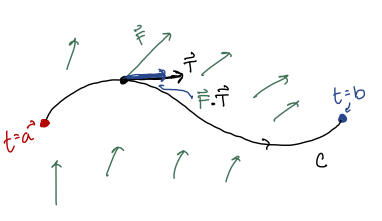
\includegraphics[width=\textwidth]{Ch13s2-Work.png}

%%\end{minipage}
\hspace*{.4in}
%\begin{minipage}{.6\textwidth}

A curve  \(C\) can be parametrized using a \textbf{vector function}:
\[
\vec{r}(t) = \<x(t), y(t)\>, \qquad \qquad a\leq t \leq b
\]
Tangent Vector:
\[
\vec{r}\ '(t) = \<x'(t), y'(t))\>
\]
Unit Tangent Vector:
\[
\vec{T}(t) = \frac{\vec{r}\ '(t)}{|\vec{r}\ '(t)|} 
\]
Work:
\[
W = \vec{F}\cdot\vec{D} = |\vec{F}||\vec{D}|\cos\theta = F_D|\vec{D}|
\]

%%\end{minipage}

\vspace*{.1in}%\hrule \vspace*{.2in}

\subsection*{Line Integrals over Vector Fields: Work}
%
%\[
%\int_C \vec{F}\cdot d\vec{r} 
%\]
This type of line integral represents the work done by a force \(\vec{F}\) to move a particle along the curve \(C\) from \(t=a\) to \(t=b\):

\[
W=\int_C \vec{F}\cdot d\vec{r}  = \int_a^b \vec{F}(\vec{r}(t))\cdot \vec{r}\ '(t)\ dt  = \int_C \vec{F}\cdot \vec{T}\ ds
\]

If \(\vec{F} = \left\langle P(x,y), Q(x,y)\right\rangle\) and \(d\vec{r} = \left\langle dx, dy\right\rangle\), then 
\[
\int_C \vec{F}\cdot d\vec{r} = \int_C P(x,y)\ dx + Q(x,y)\ dy 
= \int_a^b P( x(t), y(t) )\ x'(t) + Q( x(t), y(t) )\ y'(t)\ dt
\]


%\end{framed}

%%\end{minipage}
~\\~\\
\textbf{Discussion:} Geometric Implications of \(W =\int_C \vec{F}\cdot d\vec{r}\) \hfill
\textit{(See diagrams on the next page)}


%\pagebreak

\vspace*{-.2in}
\section*{Example:}


\begin{enumerate}[{Example} 1: ]
\item We will integrate \(\vec{F} = \< x^2,-xy\>\) and \(\vec{G} = \<y, x+2y\>\) along the paths shown below, which both start at \((1,0)\) and end at \((0,1)\).\\ Note that \(C_1 = C_{11} + C_{12}\) is made up of two line segments, and \(C_2\) is an arc of a circle.


%\begin{minipage}{.4\textwidth}
%\hspace*{-.5in}
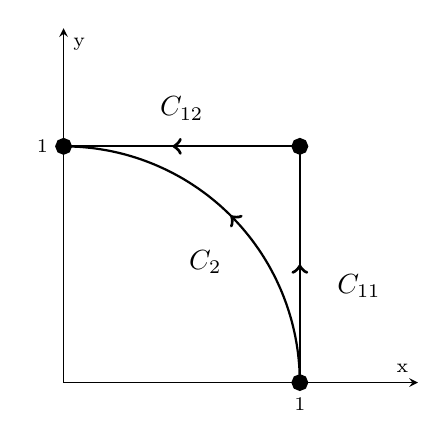
\begin{tikzpicture}
\begin{axis}[
	y=3cm,
    x=3cm,
	axis x line=middle,
	axis y line = middle,
	xmin=0,xmax=1.5,
	ymin=0,ymax=1.5,
    grid=none,
%    ticks=none,
%    yticklabels={},
%    xticklabels={},
    xtick={0,1},
    ytick={0,1},
%    xticklabels={-1,0,1},
%    yticklabels={-1,0,1},
    xlabel=x,
    ylabel=y,
    label style={font=\scriptsize},
    tick label style={font=\scriptsize}
]

\addplot[thick,black, domain=0:90, smooth, decoration = {markings,
    mark = at position .5 with {\arrow[line width=1.2pt]{>}}
  }, postaction = decorate] (cos x,sin x);
  
  \addplot[domain=0:1,thick, decoration = {markings,
    mark = at position 0.5 with {\arrow[line width=1.2pt]{>}}
  }, postaction = decorate] (1,x);
  
    \addplot[domain=0:1,thick, decoration = {markings,
    mark = at position 0.5 with {\arrow[line width=1.2pt]{<}}
  }, postaction = decorate] (x,1);



\addplot[black,only marks, mark=*, line width=2pt] coordinates{(1,0)(0,1)(1,1)};
\node [below] at (axis cs:  .6,.6) {$C_2$};
\node [below] at (axis cs:  1.25,.5) {$C_{11}$};
\node [below] at (axis cs:  .5,1.25) {$C_{12}$};

\end{axis}
%\filldraw[fill=green!20,draw=green!50!black] (1.5cm,0cm) -- (3.75cm,0cm) arc
%(0:45:3.75cm) -- (1.065cm,1.065cm) arc (45:0:1.5cm) -- cycle;
%
%

\end{tikzpicture}
%%\end{minipage}

\vfill

%\textit{Followup Discussion: Does this represent something that we can visualize?}


\end{enumerate}
\pagebreak

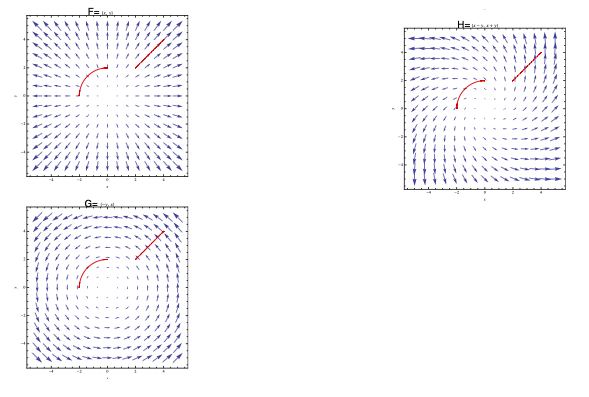
\includegraphics[angle=90,width=\textwidth]{Ch13s3-Vector-Fields-Work.png}

\pagebreak

\section*{6.3 - The Fundamental Theorem of Calculus for Line Integrals (FTCFLI)}


\hspace*{-.8in}%\begin{minipage}{1.25\textwidth}
%\begin{framed}

\subsection*{Path Dependence Terminology:}

Consider a line integral over a vector field from a starting point \(A\) to and ending point \(B\):
\[
\int_C \vec{F}\cdot d\vec{r}
\]

If the value of the line integral changes depending on what path is taken from \(A\) to \(B\), then we say that it is \textbf{path dependent}.\\
 If the value of the line integral is the same for any path between \(A\) and \(B\), then we say that it is \textbf{path independent}.
~\\
%A vector field \(\vec{F}\) is called \textbf{conservative} if
%\[
%\vec{F} = \grad f.
%\]
%for some scalar function \(f\), which is called the \textbf{potential function} for \(\vec{F}\).

\vspace*{.1in}%\hrule \vspace*{.2in}

\subsection{FTCFLI:}
If \(f\) is differentiable and \(\grad f\) is continuous on a curve \(C\) parametrized as \(\vec{r}(t)\) for \(a\leq t \leq b\), then

\[
\int_C \grad f \cdot d\vec{r} = f(\vec{r}(b)) - f(\vec{r}(a)).
\]

This means that if \(\vec{F}=\grad f\) for some potential function \(f\) then the line integral \(\int_C \vec{F}\cdot d\vec{r}\) is path independent.

%\end{framed}

%%\end{minipage}

\section*{Example:}


\begin{enumerate}[{Example} 1: ]
\addtocounter{enumi}{1}
\item Evaluate \(\int_C \vec{F}\cdot d\vec{r}\) for \(\vec{F} = \<2xy, x^2\>\) and \(C\) shown below:\\

%\begin{minipage}{.4\textwidth}
%\hspace*{-.5in}
\begin{tikzpicture}
\begin{axis}[
	y=2cm,
    x=2cm,
	axis x line=middle,
	axis y line = middle,
	xmin=-1.5,xmax=2.5,
	ymin=-1.5,ymax=1.5,
    grid=none,
%    ticks=none,
%    yticklabels={},
%    xticklabels={},
    xtick={-1,0,1,2},
    ytick={-1,0,1},
%    xticklabels={-1,0,1},
%    yticklabels={-1,0,1},
    xlabel=x,
    ylabel=y,
    label style={font=\scriptsize},
    tick label style={font=\scriptsize}
]

\addplot[domain=-1:0,thick, samples=100,decoration = {markings,
    mark = at position 0.5 with {\arrow[line width=1.2pt]{>}}
  }, postaction = decorate]{sqrt(1-(x)^2)};
  
\addplot[domain=0:2,thick, samples=100,decoration = {markings,
    mark = at position 0.5 with {\arrow[line width=1.2pt]{>}}
  }, postaction = decorate]{sqrt(1-(x)^2/4)};
  
\addplot[domain=2:0,thick, decoration = {markings,
    mark = at position 0.5 with {\arrow[line width=1.2pt]{>}}
  }, postaction = decorate] {x/2-1};



\addplot[black,only marks, mark=*, line width=2pt] coordinates{(-1,0)(0,1)(2,0)(0,-1)};
\node [below] at (axis cs:  -1,1.25) {$x^2+y^2=1$};
\node [below] at (axis cs:  1.5,1.25) {$\tfrac{x^2}{4}+y^2=1$};

\end{axis}
%\filldraw[fill=green!20,draw=green!50!black] (1.5cm,0cm) -- (3.75cm,0cm) arc
%(0:45:3.75cm) -- (1.065cm,1.065cm) arc (45:0:1.5cm) -- cycle;
%
%

\end{tikzpicture}
%%\end{minipage}

\end{enumerate}

\pagebreak


\section*{Group Work:}

Evaluate the line integral \(\int_C 2x\cos y\ dx - x^2\sin y\ dy\) for the curves described below. \\
%\textit{Hint:} Start by parametrizing the curves \(C_1\) and \(C_2\).

%\begin{minipage}{.4\textwidth}
%\hspace*{-.5in}
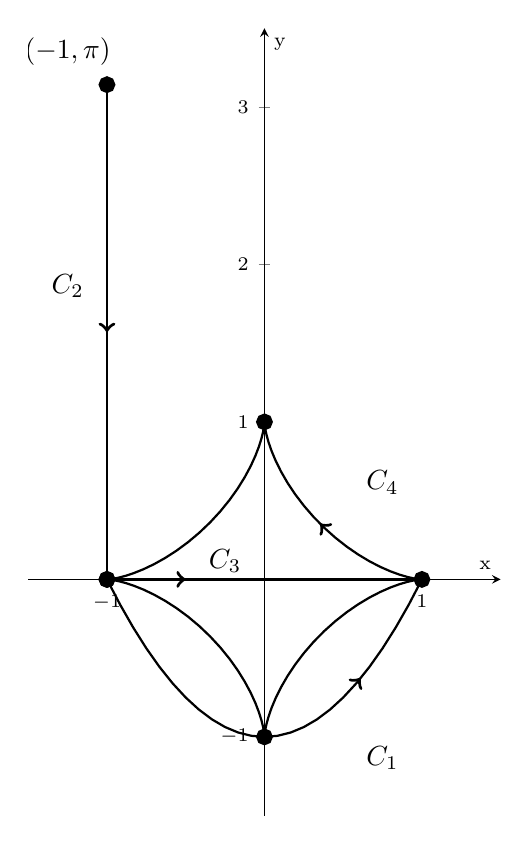
\begin{tikzpicture}
\begin{axis}[
	y=2cm,
    x=2cm,
	axis x line=middle,
	axis y line = middle,
	xmin=-1.5,xmax=1.5,
	ymin=-1.5,ymax=3.5,
    grid=none,
%    ticks=none,
%    yticklabels={},
%    xticklabels={},
    xtick={-1,0,...,1},
    ytick={-1,0,...,3},
%    xticklabels={-1,0,1},
%    yticklabels={-1,0,1},
    xlabel=x,
    ylabel=y,
    label style={font=\scriptsize},
    tick label style={font=\scriptsize}
]

\addplot[domain=0:2*pi,thick, samples=100,decoration = {markings,
    mark = at position 0.125 with {\arrow[line width=1.2pt]{>}}
  }, postaction = decorate]({cos(deg(x))^3},{sin(deg(x))^3});
  
  \addplot[domain=pi:0,thick, decoration = {markings,
    mark = at position 0.5 with {\arrow[line width=1.2pt]{>}}
  }, postaction = decorate] (-1,x);
  
    \addplot[domain=-1:1,thick, decoration = {markings,
    mark = at position 0.25 with {\arrow[line width=1.2pt]{>}}
  }, postaction = decorate] (x,0);
  
    \addplot[domain=-1:1,thick, decoration = {markings,
    mark = at position 0.75 with {\arrow[line width=1.2pt]{>}}
  }, postaction = decorate] {x^2-1};



\addplot[black,only marks, mark=*, line width=2pt] coordinates{(-1,0)(0,1)(-1,pi)(1,0)(-1,0)(0,-1)};
\node [below] at (axis cs:  .75,.75) {$C_4$};
\node [below] at (axis cs:  -.25,.25) {$C_3$};
\node [below] at (axis cs:  -1.25,2) {$C_2$};
\node [below] at (axis cs:  .75,-1) {$C_1$};
\node [below] at (axis cs:  -1.25,3.5) {$(-1,\pi)$};

\end{axis}
%\filldraw[fill=green!20,draw=green!50!black] (1.5cm,0cm) -- (3.75cm,0cm) arc
%(0:45:3.75cm) -- (1.065cm,1.065cm) arc (45:0:1.5cm) -- cycle;
%
%

\end{tikzpicture}
%%\end{minipage}
%
%\begin{minipage}{.6\textwidth}
\begin{enumerate}[(a)]

\item \(C_1\): parabola \(y=x^2-1\) from \((-1,0)\) to \((1,0)\)
\item \(C_2\): line segment from \((-1,\pi)\) to \((-1,0)\)
\item \(C_3\): \(x\) axis from \((-1,0)\) to \((1,0)\)
\item \(C_4\): the astroid \(\vec{r}(t)=\<\cos^3 t, \sin^3 t\>\) for \(0\leq t\leq 2\pi\)

\vspace*{2in}

\end{enumerate}
%%\end{minipage}

\vfill
%\pagebreak


\end{document}